\documentclass[uplatex,dvipdfmx,a4paper,11pt]{jsarticle}

\usepackage[top=25mm,bottom=25mm,left=25mm,right=25mm]{geometry}
\usepackage{array}
\usepackage{tabularx}
\usepackage{booktabs}
\usepackage{enumitem}
\usepackage{graphicx}

\setlength{\parindent}{0pt}
\setlength{\parskip}{0.6em}

\usepackage{titlesec}
\titleformat{\section}
  {\normalfont\Large\bfseries}{\thesection.}{0.6em}{}
\titleformat{\subsection}
  {\normalfont\large\bfseries}{\thesubsection}{0.6em}{}
\titlespacing*{\section}{0pt}{1.2em}{0.6em}
\titlespacing*{\subsection}{0pt}{1.0em}{0.4em}

\newcommand{\sectionrule}{\par\medskip\noindent\rule{\linewidth}{0.6pt}\par\medskip}

\renewcommand{\labelitemi}{\textbullet}
\renewcommand{\labelitemii}{\textopenbullet}
\setlist[itemize]{leftmargin=1.6em,itemsep=0.1em,topsep=0.2em}
\setlist[enumerate]{leftmargin=2.0em,itemsep=0.1em,topsep=0.2em}

\providecommand{\textopenbullet}{\ensuremath{\circ}}

\begin{document}

{\LARGE\bfseries 作業ログ}\par\bigskip

報告者：梅澤颯太

報告日：2026年6月30日

プロジェクト名：タクトーン～IMU ジェスチャーで奏でるArduino オーケストラ～

\sectionrule

\section{進捗サマリー（要約）}

\begin{itemize}
  \item 全体進捗率：95\%
  \item マイルストーン達成状況：ガントチャートに載っている個人のタスクは全て完了
  \item 主要成果：
    \begin{itemize}
      \item 過去に作成されたドキュメントサイトを，現行システムの構成に合わせて再編した．
      \item システム，実装，開発履歴の各ページを整理し，必要な情報へ到達しやすいサイドバー構成に更新した．
    \end{itemize}
  \item 課題：
    \begin{itemize}
      \item ページ構成を大きく変更したため，リンク切れや説明の重複がないか最終確認する必要がある．
      \item 発表後も参照できる資料にするため，実機検証の結果や最終仕様との不一致を継続して修正する必要がある．
    \end{itemize}
\end{itemize}

\subsection{ガントチャート}

\begin{figure}[htbp]
  \centering
  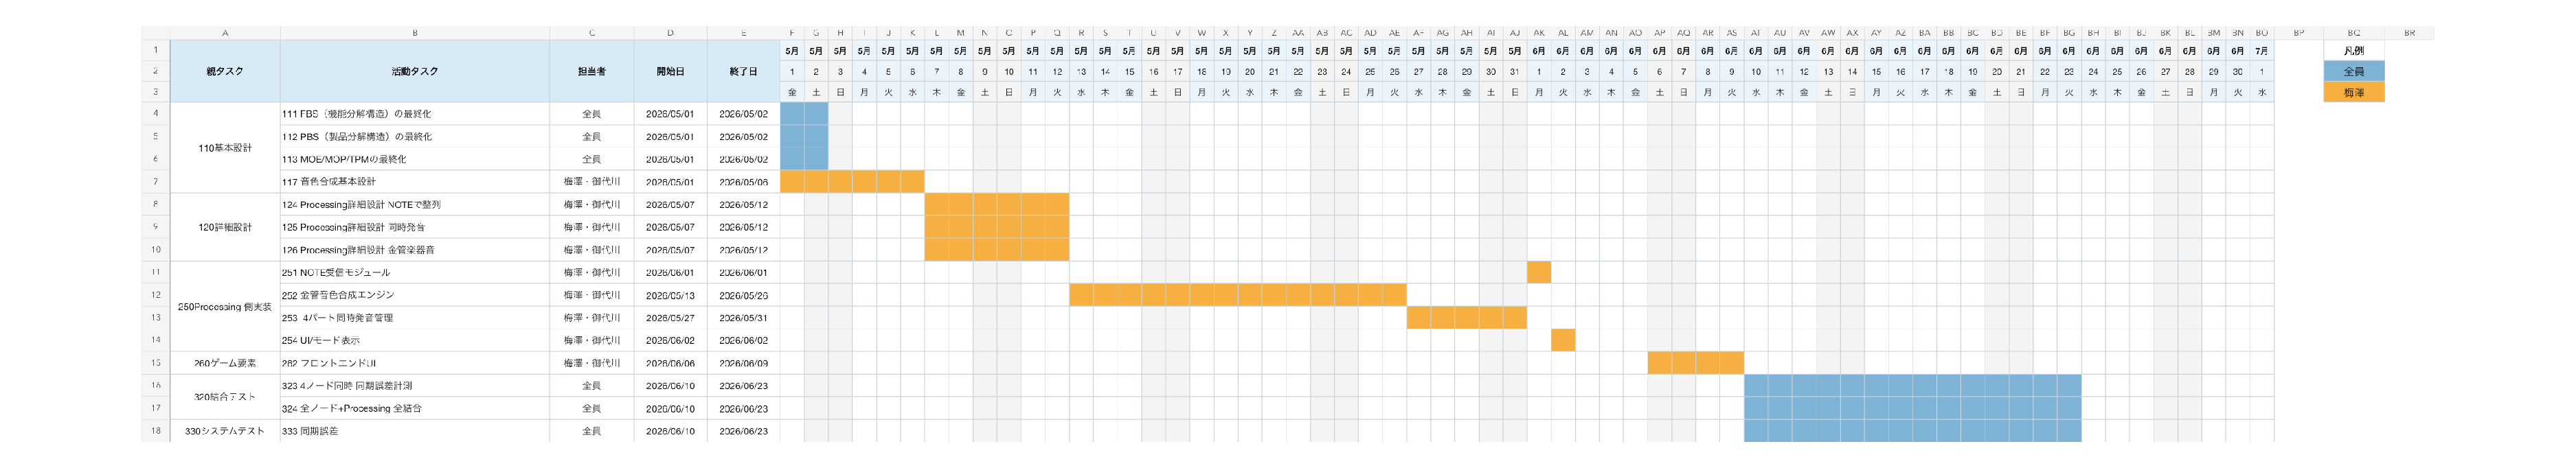
\includegraphics[width=\linewidth]{fig/ガントチャート_梅澤_全員.pdf}
  \caption{全体のガントチャート}
\end{figure}

\sectionrule

\section{作業ログ（詳細トラッキング）}

\begin{tabularx}{\linewidth}{@{}p{0.16\linewidth}p{0.12\linewidth}XX@{}}
\toprule
日付 & 作業時間 & 作業内容 & 成果・メモ \\
\midrule
2026/06/29 & 1.5h & ドキュメントサイトの構成と内容を更新した． & 現行システム，実装解説，開発履歴を軸にページを再編し，サイドバー，数式表示，ファームウェアおよびPCアプリの解説を現行仕様に合わせて整理した． \\
\bottomrule
\end{tabularx}

\sectionrule

%================================================================
% 3. 課題管理
%================================================================
\section{課題管理}

\begin{tabularx}{\linewidth}{@{}p{0.20\linewidth}Xp{0.08\linewidth}p{0.08\linewidth}Xp{0.11\linewidth}p{0.09\linewidth}@{}}
\toprule
課題 & 発生原因 & 影響度 & 優先度 & 対策 & 期限 & 状態 \\
\midrule
サイト内リンクの最終確認 & ページの追加，削除，移動を伴う大規模な再編を行った． & 高 & 高 & サイトをビルドし，リンク切れとサイドバーからの到達性を確認する． & 発表前 & 対応予定 \\
最終仕様との整合確認 & 開発終盤にもファームウェアとPCアプリの調整が続いている． & 中 & 中 & 実機検証結果と最終コードを基準に，数値や状態遷移の説明を見直す． & 最終提出前 & 対応予定 \\
\bottomrule
\end{tabularx}

\sectionrule

%================================================================
% 4. AI利用状況と検証
%================================================================
\section{AI利用状況と検証（再現性重視）}

\subsection{利用内容}

\begin{itemize}
  \item 利用目的：作業ログ文章の作成補助
  \item 入力（プロンプト要旨）：
    \begin{itemize}
      \item 前週の作業ログを参考に，同じ構成で今週分の作業ログを作成するよう依頼した．
      \item 6月29日に1時間30分かけてドキュメントサイトを更新したことを伝えた．
      \item Gitの変更履歴から，実際に更新したページ構成と機能を確認するよう依頼した．
    \end{itemize}
  \item 出力概要：
    \begin{itemize}
      \item 前週の形式に合わせて，進捗サマリー，作業ログ，課題管理，AI利用状況，次回計画を整理した．
    \end{itemize}
\end{itemize}

\sectionrule

\subsection{検証方法}

\begin{itemize}
  \item 検証手法：
    \begin{itemize}
      \item 作業ログの日付，作業時間，作業内容を実際の記録およびGitの変更履歴と照合する．
      \item 生成したPDFを画像化し，文字化け，表のはみ出し，図の欠落がないか確認する．
    \end{itemize}
  \item 検証手順：
    \begin{enumerate}
      \item 6月29日のコミット内容と作業ログの記述を比較する．
      \item 作業時間が1時間30分と記載されていることを確認する．
      \item TeXを再コンパイルし，全ページのレイアウトを目視確認する．
    \end{enumerate}
\end{itemize}

\sectionrule

\subsection{ファクトチェック結果}

\begin{itemize}
  \item 一致点：
    \begin{itemize}
      \item 作業日，作業時間，サイト構成の再編，サイドバー更新は実際の作業内容と一致していた．
    \end{itemize}
  \item 不一致・疑義：
    \begin{itemize}
      \item なし
    \end{itemize}
  \item 最終判断：
    \begin{itemize}
      \item レポート本文として採用する．
    \end{itemize}
  \item 根拠：
    \begin{itemize}
      \item 本人が提示した作業時間とGit上で確認できる変更内容を基に記述しているため．
    \end{itemize}
\end{itemize}

\sectionrule

%================================================================
% 5. 次回計画
%================================================================
\section{次回計画}

\begin{itemize}
  \item 目標：
    \begin{itemize}
      \item ドキュメントサイトをビルドし，リンク切れや表示崩れがないことを確認する．
      \item 発表と実機検証で確定した内容をドキュメントへ反映する．
    \end{itemize}
  \item 達成基準：
    \begin{itemize}
      \item 全ページがビルドでき，サイドバーから主要ページへ移動できること．
      \item 現行システムの台数，通信方式，状態遷移，演奏仕様が最終コードと一致していること．
    \end{itemize}
  \item 期限：
    \begin{itemize}
      \item 最終提出前
    \end{itemize}
\end{itemize}

\sectionrule

%================================================================
% 6. その他
%================================================================
\section{その他}

\begin{itemize}
  \item 今週は，仕様の確認や現在のシステムの理解を目的として，ドキュメントサイトの内容を整理した．
  \item ページ数を増やすことではなく，現行システム，実装方法，詳細仕様，開発履歴という読み手の目的別に情報を分けることを重視した．
\end{itemize}

\sectionrule

%================================================================
% 7. 付録
%================================================================
\section{付録}

無し

\end{document}
